\chapter{Related Works}
In this chapter, related work on the relevant topics of this work is presented and discussed. The topics include autonomous negotiation, multi-agent reinforcement learning. At the last section, the work of reinforcement learning used in autonomous negotiation is presented. 

\section{Heuristic Negotiation Strategies for Autonomous Negotiation}
\subsection{Time-based Strategy (Aspiration Negotiator)}
Aspirations are the specific goals in a negotiation that a negoitator wishes to achieve as part of an agreement. Empricial evidence has shown that negotiators with higher aspirations tend to achieve better bargaining results. First, aspiration of negotiator can help to determine the outer limit of what negotiator will request. Second, optimistic aspirations can make the negotiators to work harder\parencite{Schneider2004}. Many aspiration negotiators are time dependent, such as Boulware(with concession factor $e=1/2$), Hardliner($e=0$), Conceder Linear($e=1$) and Conceder($e=2$)\parencite{FARATIN1998159}. Boulwarism is the tactic of making a "take-it-or-leave-it" offer in a negotiation, with no further concessions or discussion. It was named after General Electric's former vice president Lemuel Boulware, who promoted the strategy\parencite{William1991}.

The value of issue $j$ as the offer at time $t$ sent by agent a to agent b is modeled as follows:
\begin{equation}
x_{a \rightarrow b}^{t}[j]=\left\{\begin{array}{ll}
\min _{j}^{a}+\alpha_{j}^{a}(t)\left(\max _{j}^{a}-\min _{j}^{a}\right) & \text { if } V_{j}^{a} \text { is decreasing } \\
\min _{j}^{a}+\left(1-\alpha_{j}^{a}(t)\right)\left(\max _{j}^{a}-\min _{j}^{a}\right) & \text { if } V_{j}^{a} \text { is increasing. }
\end{array}\right.
\end{equation}
Where $V_{j}$ denotes utility value of issue $j$ set as the offer, $\min _{j}$ and $\max _{j}$ mean the minimum and maximum value of offer $j$, respectively.

Figure \ref{fig:boulware-conceder} diagrams the convexity degree of $\alpha_j(t)$ used in the calcualtion model of offer's value.

\begin{figure}[htbp]
\centering
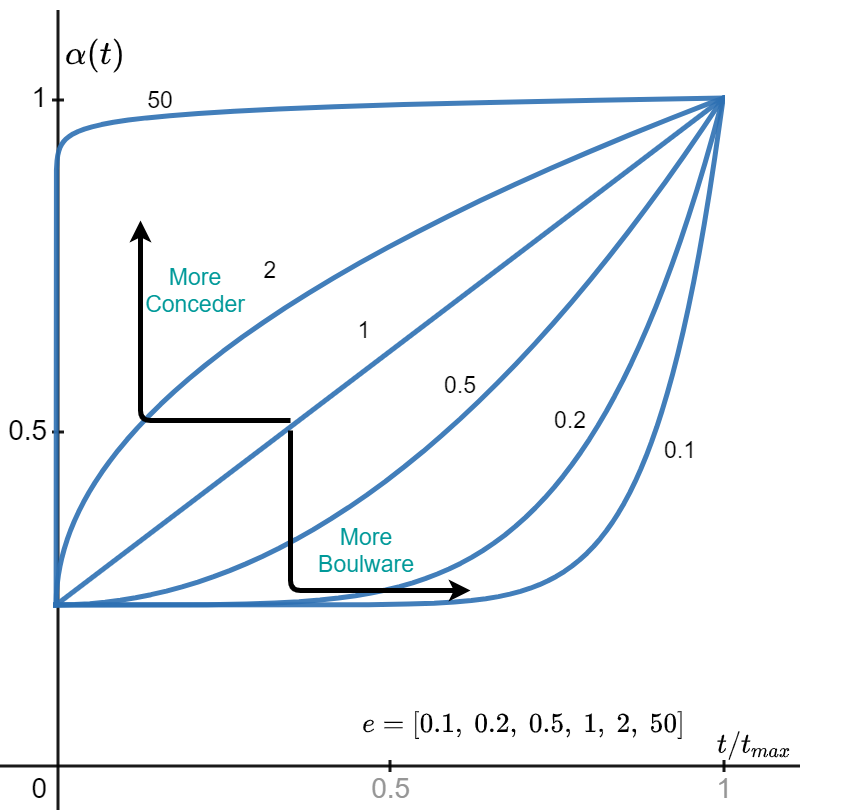
\includegraphics[width=0.6\textwidth]{./images/boulware-conceder.png}
\caption{Computation of $\alpha(t)$. Time is presented as relative to $t_{max}$. Polynomial Function: $\alpha_{j}(t)=\kappa_{j}+\left(1-\kappa_{j}\right)\left(\min \left(t, t_{\max }\right) / t_{\max }\right)^{1 / e}$. $\kappa_{j}$ is minimum conceder of negotiator.}
\label{fig:boulware-conceder}
\end{figure}

The offer will always between the value range($[min_j, max_j]$), the initial constant will be given at the beginning, and before the deadline is reached, the strategy will suggest to provide a reserved value.

\subsection{Tit for tat strategies}

\subsection{Concurrent Negotiation Strategy (\gls{cns})}
In a concurrent negotiation environment, an agent will negotiate with many opponents at the same time(one-to-many). One issue is how to coordinate all these negotiations. The author of the paper \parencite{Williams12Concurrent} designed an intuitive model with two key parts, namely the \texttt{Coordinator} and \texttt{Negotiation Thread} to deal with this problem.

\begin{figure}[htbp]
\centering
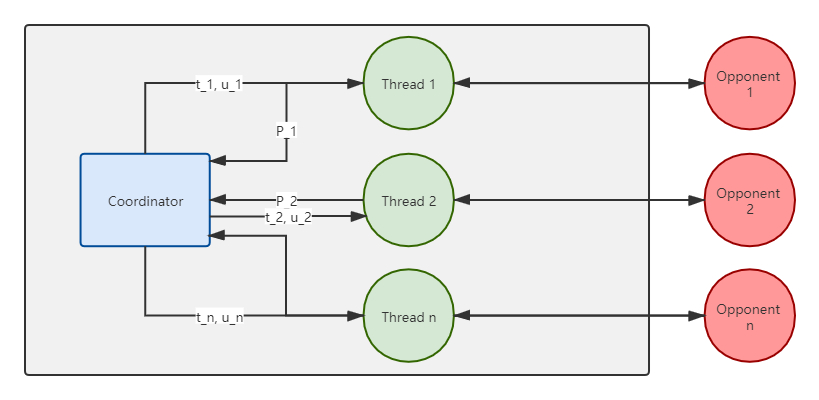
\includegraphics[width=0.8\textwidth]{./images/heuristic_concurrent_negotiation.png}
\caption{Architecture of the concurrent negotiation agent, best time: $t_i$ and utility value: $u_i$, probability distributions: $P$ \parencite{Williams12Concurrent}.}
\label{fig:heuristic-concurrent-negotiation}
\end{figure}

\textbf{Negotiation Threads:}The strategy of each negotiation thread is an extension of a recently published, principled, adaptive bilateral negotiation agent. This agent was designed to be used in a similarly complex environment, but only for negotiations against a single opponent.

\textbf{Coordinator:}The role of the coordinator is to calculate the best time, $t_i$ and utility value, $u_i$ at that time, for each thread. To do so, it uses the probability distributions received from the individual threads, which predict future utilities offered by the opponents.

%\subsection{Optimal Negotiation Strategies}
\subsection{Conclusion}
From the analysis of the heuristic negotiation strategy in a specific field, We can get some important parameters, such as time, the opponent's offer, these parameters can be regarded as important information that affects the negotiation process.

\section{Reinforcement Learning used in Autonomous Negotiation}
\textbf{\gls{negosi}:} A novel algorithm named negotiation-based MARL
with sparse interactions (NegoSI) is presented by \texttt{Luowei Zhou}. In contrast to traditional sparse-interaction based MARL algorithms, NegoSI adopts the equilibrium concept and makes it possible for agents to select the non-strict Equilibrium Dominating Strategy Profile (non-strict EDSP) or Meta equilibrium for their joint actions \parencite{L2017NegoSI}.


\textbf{\gls{rlboa}:} From the paper \parencite{Bakker2019RLBOAAM} A Modular Reinforcement Learning Framework for Autonomous Negotiating Agents. This framwork implemented an agent that used tabular Q-Learning on the compressed state and action space to learning bidding strategy which is one of modules \gls{boa} proposed in the paper \parencite{Baarslag2014}. Negotiation strategy was split into three modules: bidding strategy, the opponent model, and the acceptance strategy. \gls{rlboa} maps the multi-dimensional contract space to the utility axis, which enables compact and universal descriptions of states and actions. Hence, the action space of this framework is discrete. The model is diagrammed in the Figure \ref{fig:rlboa}.

\begin{figure}[htbp]
\centering
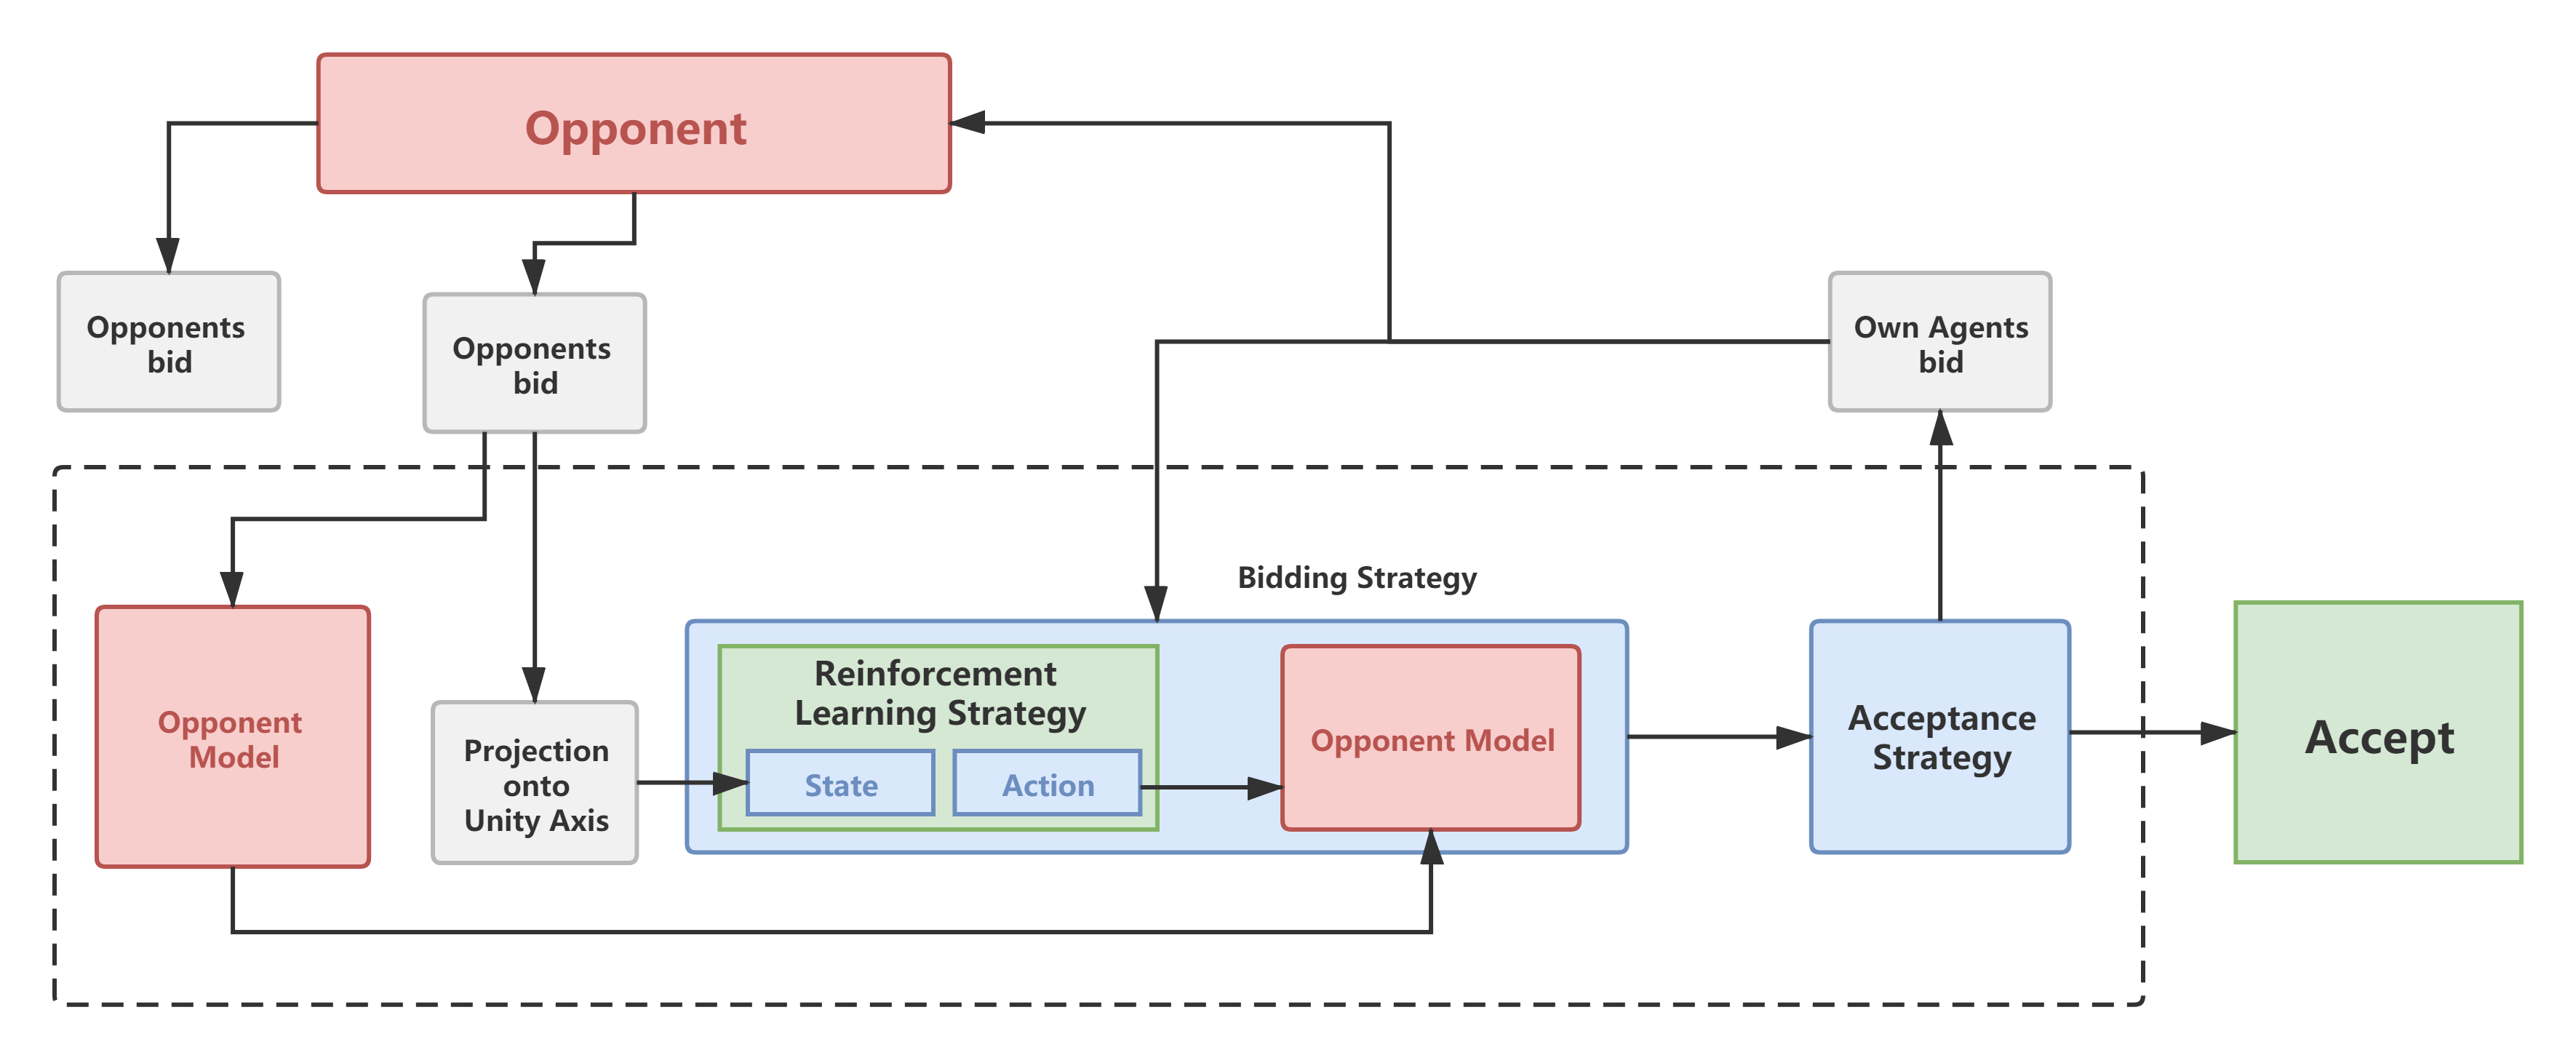
\includegraphics[width=1.0\textwidth]{./images/rlboa.png}
\caption{A schematic overview of the RLBOA-framework (within the dashed box), Source: Own illustration based
on\parencite{Bakker2019RLBOAAM}.}
\label{fig:rlboa}
\end{figure}


\textbf{\gls{anegma}:} Work by \parencite{bagga2020deep}. A novel DRL-inspired agent model called ANEGMA, which allows the buyer to develop an adaptive strategy to effectively use against its opponents (which use fixed-but-unknown strategies) during concurrent negotiations in an environment with incomplete information . The architecture of \gls{anegma} is shown in Figure \ref{fig:anegma}.
\begin{figure}[htbp]
\centering
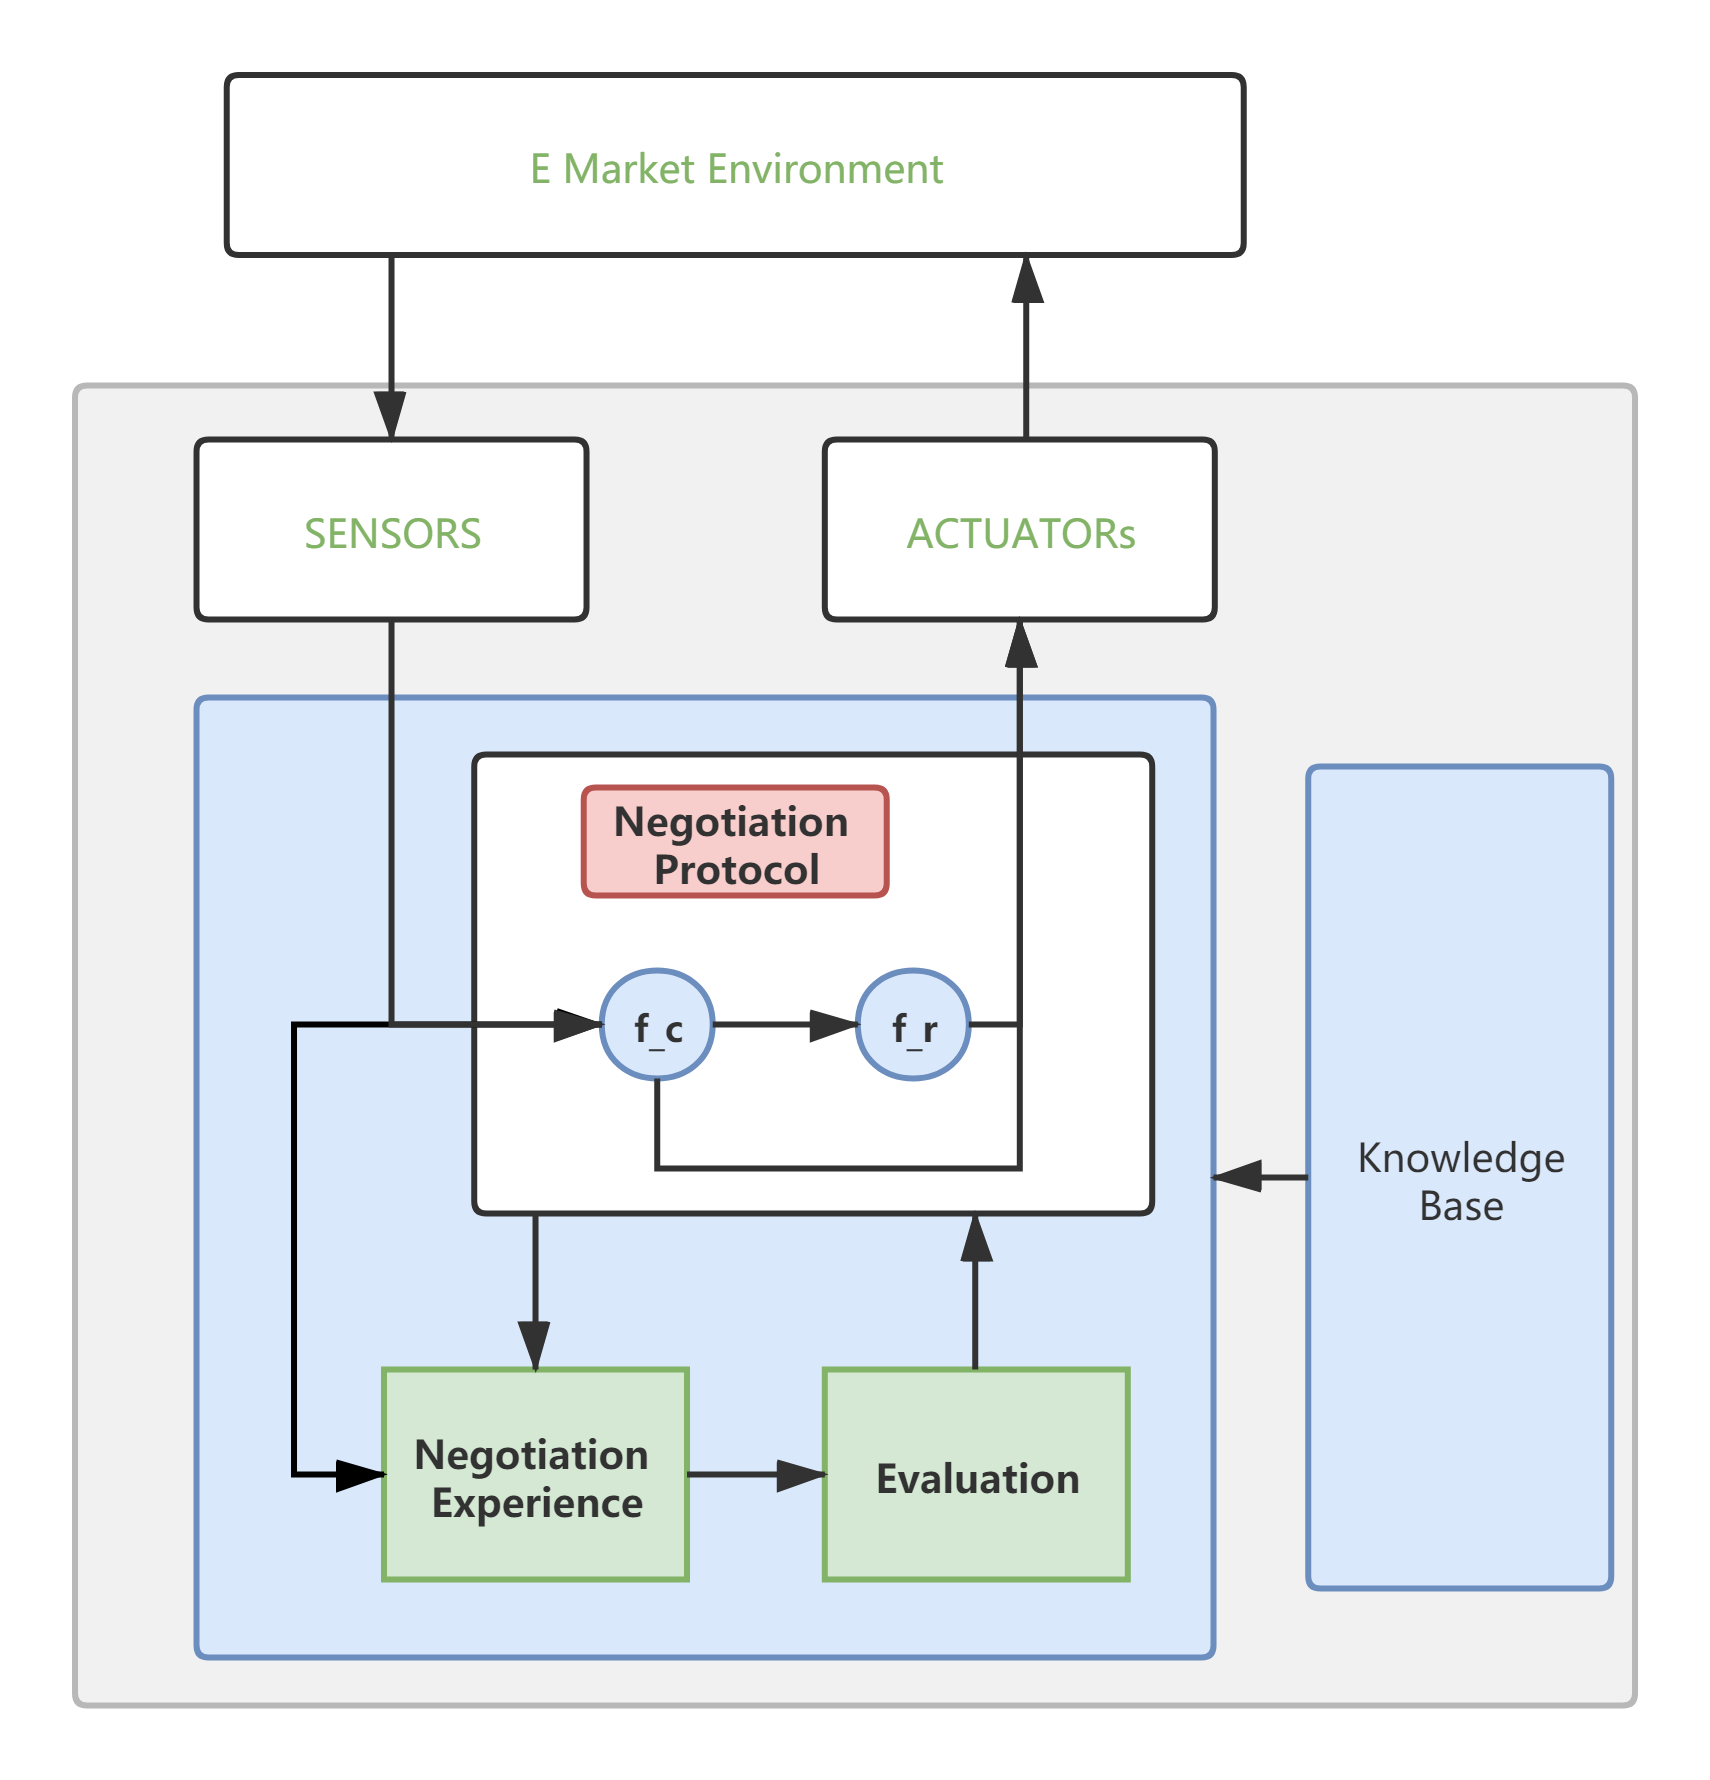
\includegraphics[width=0.6\textwidth]{./images/anegma.png}
\caption{The Architecture of \gls{anegma}. Source: Own illustration based on\parencite{bagga2020deep}.}
\label{fig:anegma}
\end{figure}


\section{Challenges in Deep Reinforcement Learning}

\subsection{Sparse Reward}
For financial problem, the reward is usually profit and an appropriate reinforcement learning signal should be based on it. When an agent learns the strategy just with it, the reward is too sparse. Hence, the reward function is needed to provide more frequent feedback or redesign the learning model. Methods \textbf{Reward Shaping},\textbf{ Curiosity Driven} and \textbf{Imitation Learning} proposed to solve sparse reward problem, will be introduced in this section.

\paragraph{Reward Shaping\parencite{Wiewiora2010}} is a method for engineering a reward function in order to provide more frequent feedback on appropriate behaviors. Providing feedback during early learning is crucial, so try promising behaviors as early as possible. This is necesary in large domains, where reinforcement signals may be few and far apart. If a method added shaping rewards in a way, it need to guarantees the optimal policy maintains its optimality. Ng et al. proposed a method with a new concept potential function $\Phi()$ to guarantee it. Hence, reward shpaing $f$ is described as $f(s, s^{\prime}) = \gamma\Phi(s^{\prime}) - \Phi(s)$ over the stats\parencite{Ng1999PolicyIU}. The form means shaping reward $f$ for transitioning from state $s^{\prime}$ to $s$ is defined as the discounted change in this state potential. Based on the value function mentioned in the section \ref{background:value-function} , the augmented value function is closely related to the original and is described as $V^{\prime}(s) = V(s) - \Phi(s)$. It is obvious to set potential function $\Phi(s) \approx V(s)$. This intuition is strengthened by results presented by Wiewiora in the paper \parencite{Wiewiora2003}. The derivation process can be found in appendix.

 
\paragraph{Curiosity Driven \parencite{pathakICMl17curiosity}} The author designed a new intrinsic reward signal that describes the agent’s familiarity with the environment. The policy outputs a sequence of actions to maximize that intrinsic reward signal. In addition to intrinsic rewards, the agent optionally may also receive some extrinsic reward from the environment. Intrinsic rewards encourage agents to actively explore the environment, instead of staying in place due to lack of reward signals.

\paragraph{Imitation Learning\parencite{DBLP:journals/corr/HesterVPLSPSDOA17}} Inverse reinforcement learning (IRL) is a different approach of imitation learning, where the main idea is to learn the reward function of the environment based on the expert’s demonstrations, and then find the optimal policy.

\subsection{Non-stationary environment}
The strategy of single agent is changed during training
Multi-agent environment is non-statinal
Multi-agent deep reinforcement learning 

\subsection{Huge action space}
Action embedding, discrete action replaced by continious action space. 